
\begin{comment}
	The objective of our case study is a comparative analysis of the two environments and to find out if there exists software performance regression between a dedicated server and the virtual environment. To analyze this, we divided our project into three research questions. Following the set up of the subject systems and data preprocessing, we used requests per minute as our independent variable and performance metrics as our dependent variables to answer our research questions. %Firstly, we observe if our models are transferable across the three chosen environments. Secondly, if the models can accurately predict counter values cross-servers. Lastly, if defect injection will generate similar performance metrics values compared   

\subsection{\textbf{Data Analysis}}
Following the data transformation, we used R \cite{R} to derive conclusions for our research questions with the help of Spearman correlation, Q-Q plots \cite{qqplots}; a graphical technique to detect if two sets of data belong to the same population, Mann-Whitney \textit{U} test \cite{mannwhitney}, and generalized linear regression models (GLM) \cite{SanFranciscoStateUniversity}. Spearman correlation is used to identify the level of association between two variables while Mann-Whitney \textit{U} test is used to verify the hypothesis that if the data sets belong to the same population.
%calculate the absolute deviation in a dataset from the median \cite{brownftest} \textcolor{red}{or instead brown forsythe test. enough already for rq1, discuss}. 
Both the aforementioned methods do not strictly assume that the ordinal data is normally distributed \cite{spearman} \cite{manutest}. Due to the size of our data, heat maps \cite{heatmaps} were used to visualize the correlations. We chose model-based analysis as they can support the automatic selection and detection of performance abnormalities between heterogeneous environments. \cite{Shang:2015:ADP:2668930.2688052}\cite{Nguyen:2012:ADP:2188286.2188344}. Contrary to the usual practice of ad-hoc selection of certain target performance metrics \cite{heger2013automated} to detect performance regression, we included the compete set of all 56 metrics to build our models. For our linear regression models, we processed our data in two steps. First, we remove any metrics that showed no variance by a R script, for example a metric which has less than 20 unique values \cite{rahm2000data}. Next, we also remove the metrics which have high correlation amongst themselves to remove any \textit{multicollinearity} present \cite{mansfield1982detecting} so that the models do not over fit based on similar predictors(performance metrics) for the load. This approach will also magnify the metric which actually contribute the most to the model. The rationale behind aforementioned steps was to clean up data that may not contribute significantly to the model \cite{Shihab:2010:UIC:1852786.1852792}. 


Once our data was organized our next step was to build the GLM using the physical and the virtual environment's performance metrics. Our models were built using the load as the dependent variable and the performance metrics as the independent variable i.e. the load is dependent on the change of values of the performance metrics. with the help. We, additionally, trained and tested our models for the same environment before using it cross-environments. This served as the benchmark for lower limit of the prediction percentage error. A model tested for the same environment was validated via ten-fold cross validation \cite{Cross_Validation} \cite{kohavi1995study}. Each fold is based on a random subset of values. The model is trained on 9 folds and tested on the $10^{th}$ fold. This is done 10 times with 10 different subsets of data each time. The accuracy of our models was determined by the percentage error of the predicted load versus the actual load values which was calculated as the absolute difference of the actual and predicted load values with respect to the actual load values.

Based on the results from the GLMs we then investigate about the metrics that are contributing the most and their respective correlation values using heat maps. Heat maps allow us to graphically view, in our case, the individual metrics and their correlation values. 

\end{comment}

In this section, we present the results of our case study. The goal of our study is to evaluate the discrepancy between performance testing results in virtual and physical environments. Shown in Section~\ref{sec:related_work}, prior research examine performance testing results in three types of approaches: 1) examining individual performance metric, 2) examining relationship among performance metrics and 3) building statistical models using performance metrics. In the rest of this section, we compare the performance testing results based on such three approaches.



\subsection{Examining individual performance metric}
\label{sec:individual}

\noindent \textbf{Approach.} 

First, we compare every individual performance metric between virtual and physical environments. Since the performance tests are conducted in different environments, intuitively the values of performance metrics are not the same. For example, the virtual environment may have higher CPU usage than the physical environment. Therefore, instead of comparing the values of each performance metric in both environments, we study whether the performance metric follow the same trend in virtual and physical environments. 

First, we plot a quantile-quantile plot (Q-Q plot)~\cite{qqplots} for every performance metric in two environments. A Q-Q plot is a plot of the quantiles of the first data set against the quantiles of the second data set. We also plot a 45-degree reference line on the Q-Q plots. If the performance metric in both environments follow the same distribution, the points on the Q-Q plots should fall approximately along this reference line. A large departure from the reference line indicates that the performance metric in virtual and physical environments come from populations with different distributions. 

Second, to quantitatively measure the discrepancy, we perform a Kolmogorov-Smirnov test~\cite{kstest} between every performance metric in virtual and physical environments. Since the values of each performance metric in both environment are not the same, we first scale the metrics based on their median values and their mean absolute deviation: 

	\[
		M_{scale}=\frac{M-\tilde{M}}{MAD(M))}		
	\]
where $M_{scale}$ is the scaled value of the metric, $M$ is the original value of the metric, $\tilde{M}$ is the median value of the metric and $MAD(M)$ is the mean absolute deviation of the metric. The Kolmogorov-Smirnov test gives a p-value as the test outcome. A p-value ≤ 0.05 means that the result is statistically significant, and we may reject the null hypothesis (i.e., two populations are from the same distribution). By rejecting the null hypothesis, we can accept the alternative hypothesis, which tells us the performance metrics in virtual and physical environments do not have the same distribution. We choose Kolmogorov-Smirnov test since it does not have any assumption on the distribution of the metrics.

Finally, we calculate the Spearman's ranking correlation between every performance metric in virtual environment and and the corresponding performance metric in physical environment, in order to assesses whether same the performance metric in two environments follow the same trend during the test. We choose Spearman's ranking correlation since it does not have any assumption on the distribution of the metrics. 

\noindent \textbf{Results.}

\textbf{Most performance metrics do not follow the same distribution in virtual and physical environments.} Figure~\ref{fig:qqds2} and \ref{fig:qqcs} show the Q-Q plots by comparing the quantiles of performance metrics from virtual and physical environments. Due to the limited space, we only present Q-Q plot for CPU User time, IO data operations/sec and memory working set for both web sever and database server. The results show that the lines on the Q-Q plot are not close to the 45-degree reference line. By looking closely on the Q-Q plots we find that the patterns of each performance metric from different subject systems are different. For example, the web cpu user time for DS2 in virtual environment shows higher values than in the physical environment in the median to high range of the distribution; while the Q-Q plot of CloudStore shows web cpu user time with higher values in the low range of the distribution. In addition, the lines of Q-Q plots for database memory working set shows completely different shape in DS2 and CloudStore. The results imply that the discrepancies between virtual and physical environments are different across subject systems.

The majority of the performance metrics have statistically significantly different distribution (p-values lower than 0.05 in Kolmogorov-Smirnov tests). We find that out of 44 metrics, 3 and 2 metrics have values with low variance during the performance tests, for DS2 and CloudStore, respectively. We cannot perform Kolmogorov-Smirnov tests on such metrics. Only 13 and 12 metrics have p-values higher than 0.05, for DS2 and CloudStore, respectively, showing statistically in-signifiant difference between the distribution in virtual and physical environments. By looking closely at such metrics, we find that these metrics either do not highly related to the execution of the subject system (e.g., web server CPU privileged time in DS2), or highly related to the workload. Since the workload between two environments are similar, it is expected that the metrics relate to the workload follow the same distribution. For example, the I/O operations are highly related with the workload. The metrics related to I/O operations may show statistically in-signifiant difference between the distribution in virtual and physical environments (e.g., web server I/O write operations per second in DS2).

%the p-values are larger than 0.05 in only X metrics. In 

 %However, even if the distributions are different, the difference can be negligible. To find out the quantitative difference between the two non-identical distributions  we used Cliff's Delta \cite{cliffsdeltajack}. We did not apply this technique on counters such as \textit{elapsed time, handle count, creating process ID, ID process, thread count} and \textit{priority base} as the do not contribute to the conclusions of the performance tests. We labeled them as NA(not applicable) in our table. The results showed that most of the performance metrics did not belong to the same distribution and have a significant difference.



%As seen in Figure 2 for the subject system DS2, the CPU user times for the web servers are closer to the line Z however the plots database servers' CPU user times are highly deviated from the same line as it not visible in the same plot. The disk IO operations/sec for the web servers gradually deviate form the line Z whereas the database server is, again, highly deviated. The same can be concluded about the memory working sets for both of our environments.
%Figure 3 shows the Q-Q plots for CloudStore. The web servers CPU user times are not congruent with the line Z. The database server CPU user times towards the tail of the plot are closer to the line Z however they still do not follow the line Z. The disk IO operations for both servers tends to follow the line Z initally but gradually moves away. Further on, the memory working set for both of our servers, as seen, are distant to the line Z.

\textbf{Most performance metrics do not have the same trend in virtual and physical environments.} Table~\ref{tab:correlationrq1} shows the Spearman correlation coefficient and corresponding p-value between the selected performance metrics as Q-Q plots. We find that the for the web server memory working set in CloudStore and the database server memory working set in D2S, there exist moderate (0.69) to strong (0.46) correlation between virtual and physical environments, respectively. By examining the metrics, we find that both metrics have a increasing trend that may be cause by memory leak. Such increasing trend may be the cause of the moderate to strong correlation. Table~\ref{tab:correlationall} shows a summary of the spearman's ranking correlation of all the performance metrics in DS2 and CloudStore. Most of the correlations either have p-values higher than 0.05 or the absolute coefficient values fall between 0 to 0.3 (low correlation).

\hypobox{Performance metrics typically do not follow the same distribution or follow the same trend in virtual and physical environments. System load metric (throughput) and some performance metrics that are correlated with system load may be exceptions.}

%If the correlation value is closer to 1 the metrics have a strong correlation and if the value is closer to 0 the metrics have a weak correlation. A negative correlation means that if one of the metrics is increasing in value, the other is decreasing. For both of our subject systems we observe that the correlation values are mostly positive and are closer to 0 representing weak correlations. This conclusion, however, is not applicable to the user times from both environments as the p-value $>$ 0.05.


%\textbf{Motivation}: Performance assurance activities are not only bounded by the idea that performance regression can only be identified relative to different versions of the software. A software system might also regress once it is transferred from one environment to another. According to the norm, practitioners often rely on performance metrics generated by the virtual environment prior to releasing it on a disparate environment. We address this question by comparing the metric values between the physical and virtual server. 

%\textbf{Approach}: As mentioned earlier in Section 3, after setting up the subject systems, we used the number of requests as our workload for the systems. A script was written to randomly alter the workload after every minute for CloudStore and every two minutes for DS2. The script was based on an underlying assumption that every unit of change in the performance metrics there will be a consequent unit of change in the workload which eventually introduced variety in our dataset. \cite{linearregression}. Subsequently, the requests per minute were mapped against the performance metrics recorded via \textit{perfmon}.

%The numerical values for requests per minute were extracted out of the web server's access logs. These requests were recorded per second and reached up to thousands in a minute, depending on the workload. We then, with the aid of a script, grouped and extracted the requests per minute for as long as the test systems were exercised. The metrics, on the contrary, were recorded every 10 seconds. A set of six records was averaged out as a minute according to the timestamps. This was called a single \textit{run}. The metrics generated for the web and database server were concatenated. Ultimately, we had a dataset consisting of 500 runs where every record represented a \textit{run}; the metrics and requests generated for a given minute. This process was carried out for both of our environments. The two datasets, to analyze any discrepancies, were then analyzed using R's Q-Q plots and \textit{cor} function.

\begin{figure}[thb]
	\centering
	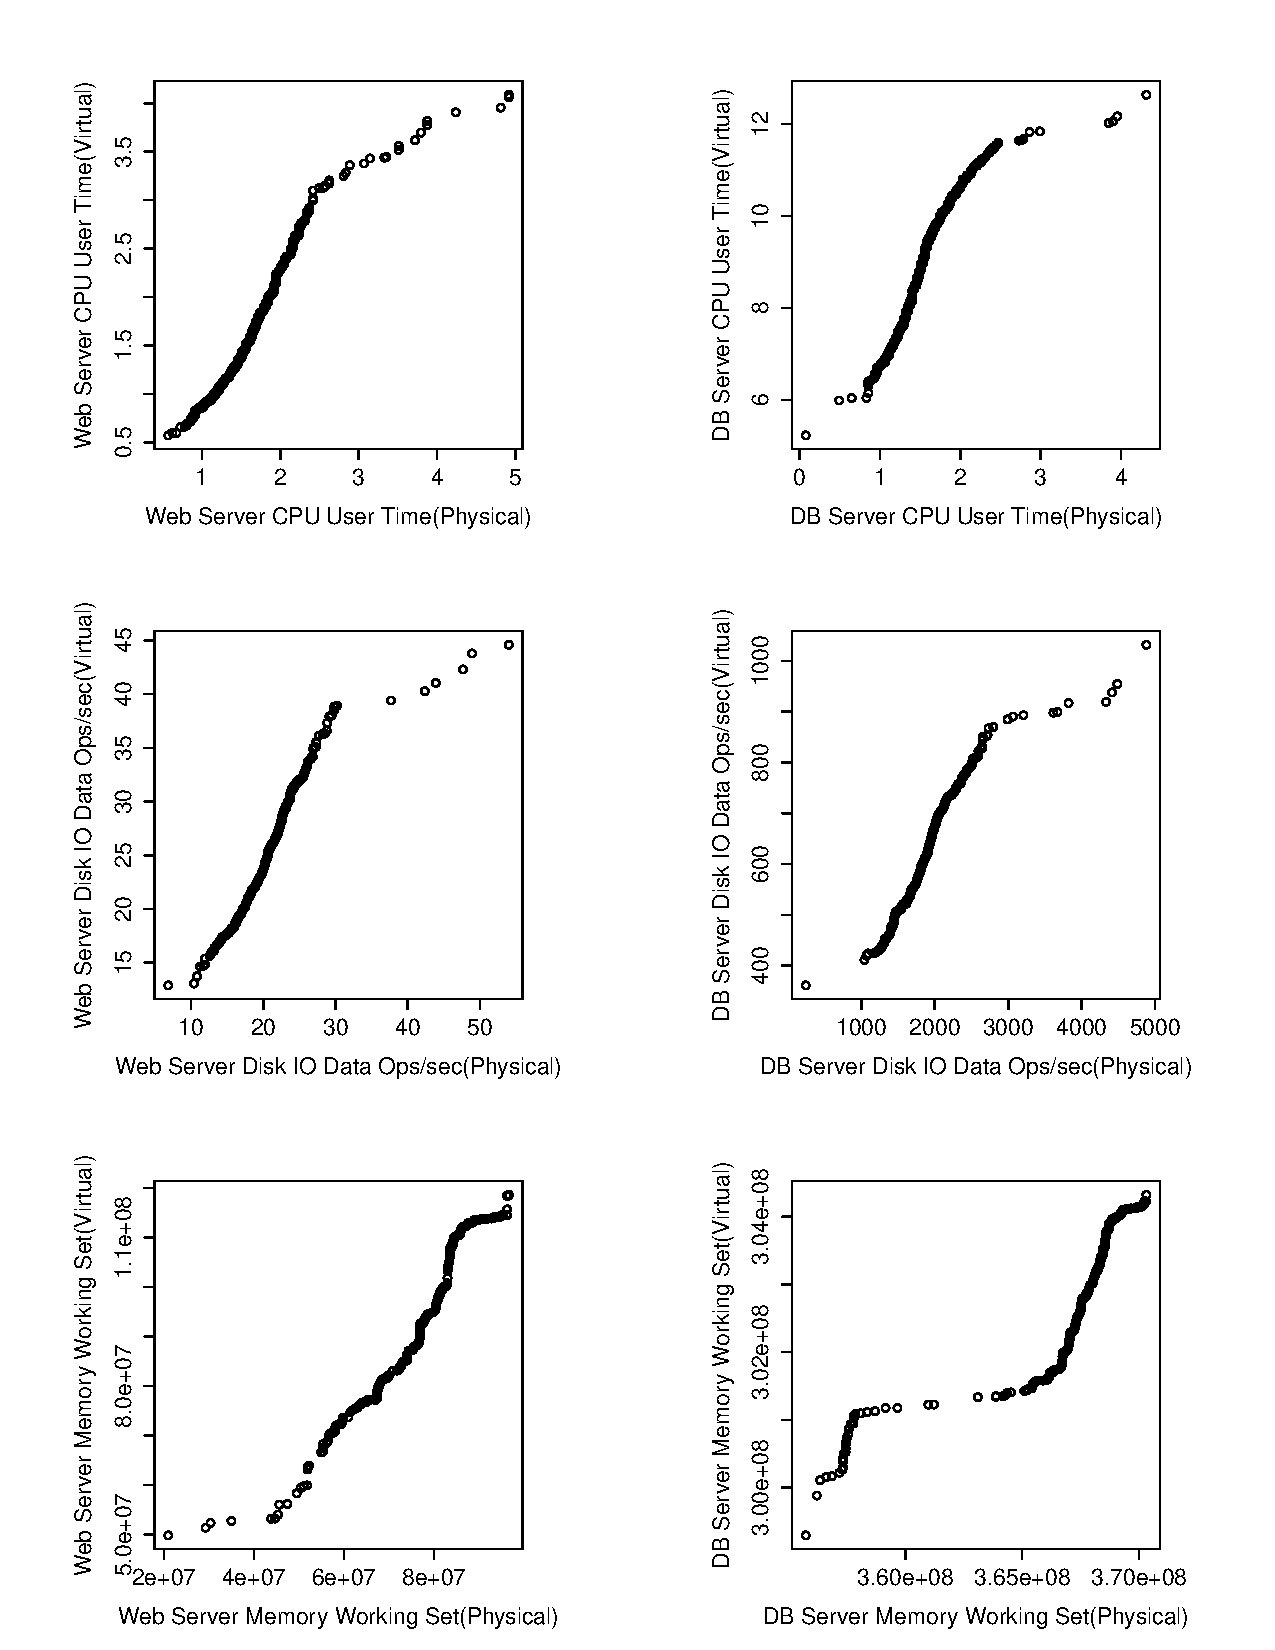
\includegraphics[width=0.9\columnwidth]{figures/qqplots_DS2.pdf}
	\caption{Q-Q plots for DS2.}
%	\captionsetup{justification=centering}
	\label{fig:qqds2}
\end{figure}



\begin{figure}[thb]
	\centering
	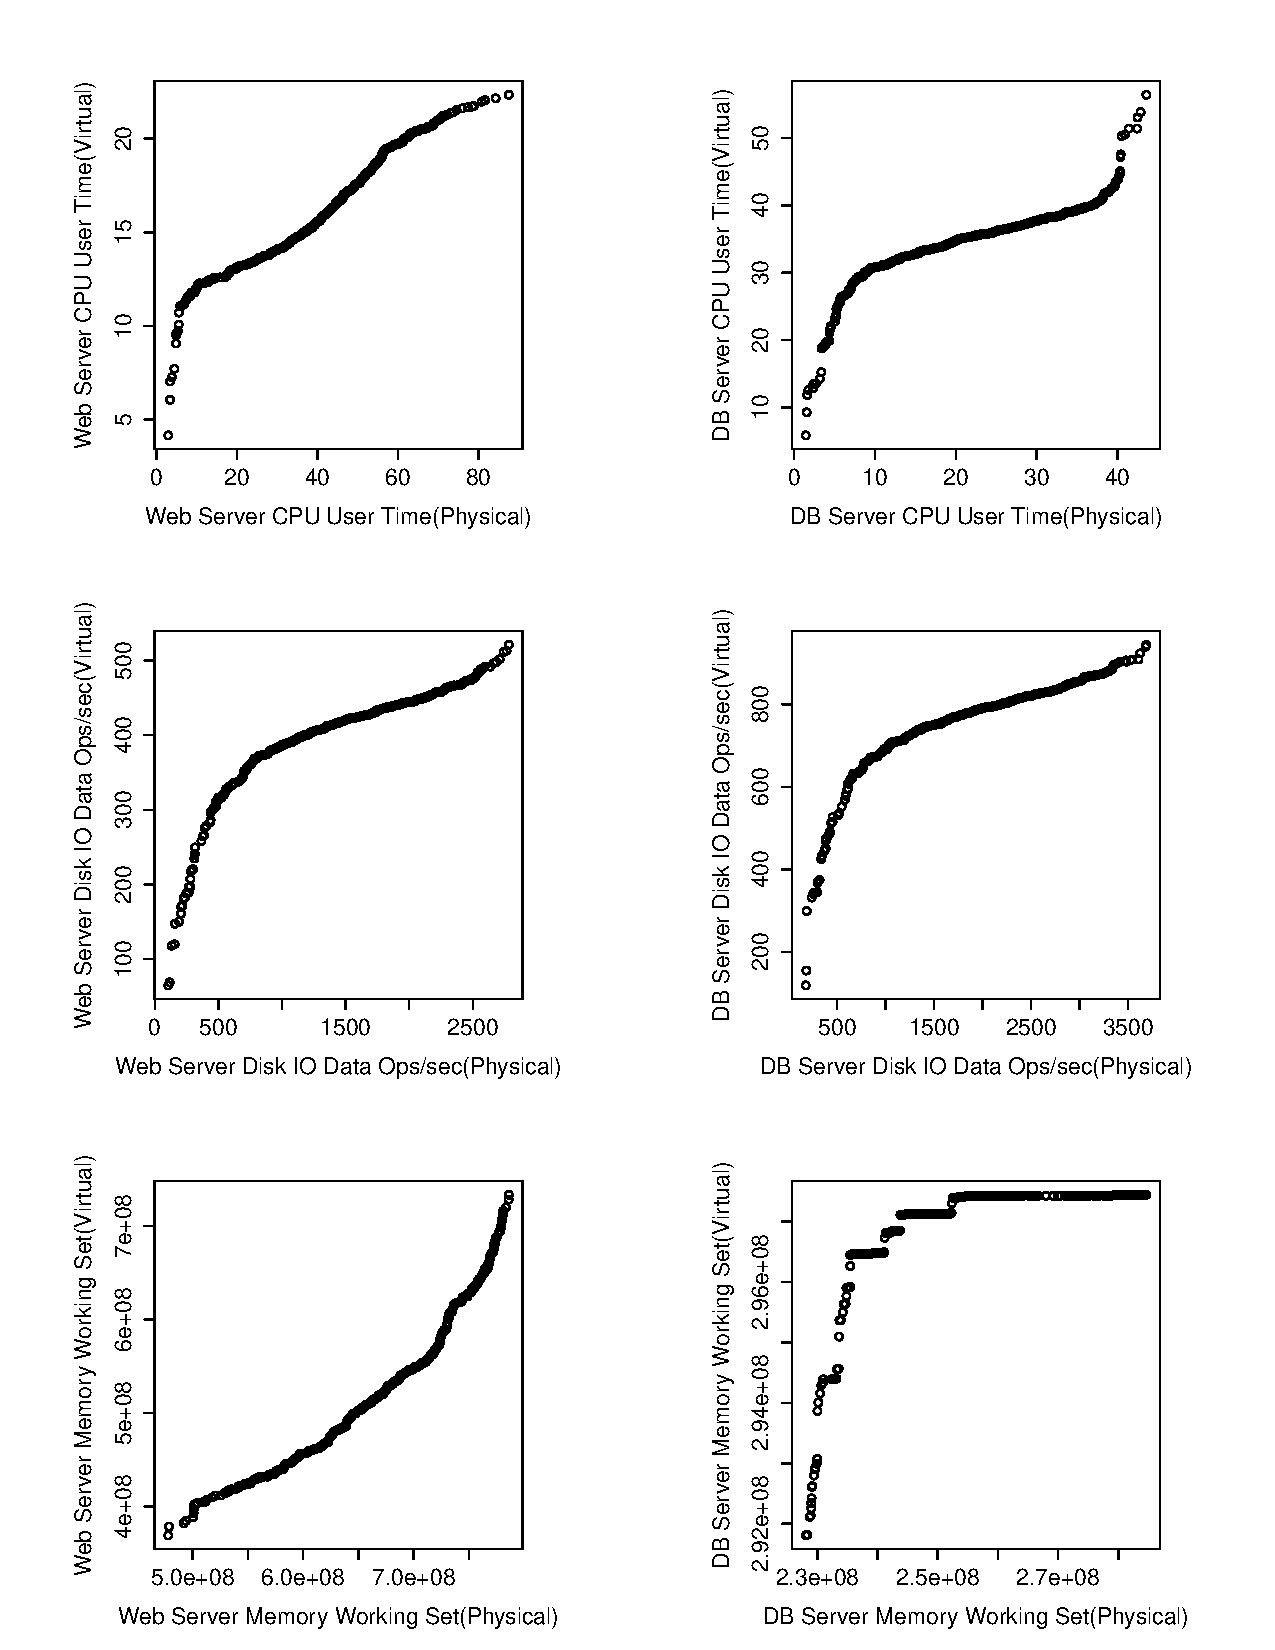
\includegraphics[width=0.9\columnwidth]{figures/qqplots_CS.pdf}
	\caption{Q-Q plots for CloudStore.}
%	\captionsetup{justification=centering}
	\label{fig:qqcs}
\end{figure}

\begin{comment}
\begin{table}[tbh]
	\centering
	\caption{Results of Ks test and Cliff Delta on Performance Metrics}
	\label{my-label}
	\resizebox{\columnwidth}{!}{%
		\begin{tabular}{|c||c|c|c|c|c|}
			\hline 
			\multirow{2}{*}{\textbf{System}} & \multirow{2}{*}{\textbf{p\textgreater0.05}} & \multicolumn{4}{c|}{\textbf{p\textless0.05}} \\ \cline{3-6} 
			&  & \textbf{Neglible} & \textbf{Small} & \textbf{Medium} & \textbf{Large} \\ %\hline
			\midrule 
			\midrule 
			DS2 & 2 & 1 & 2 & 5 & 34 \\ \hline
			CloudStore & 0 & 1 & 2 & 1 & 40 \\ \hline
		\end{tabular}%
	}
\end{table}
\end{comment}

% Please add the following required packages to your document preamble:
% \usepackage{multirow}
% \usepackage{graphicx}
\begin{table}[thb]
	\centering
	\caption{Spearman's ranking correlation coefficients and p-values of the highlighted performance metrics.}
	\label{tab:correlationrq1}
	\resizebox{\columnwidth}{!}{%
		\begin{tabular}{|c||c|c|c|c|}
			\hline
			\multirow{2}{*}{\textbf{Performance Metrics}} & \multicolumn{2}{c|}{\textbf{DS2}} & \multicolumn{2}{c|}{\textbf{CloudStore}} \\ \cline{2-5} 
			& \textbf{coef.} & \textbf{p-value} & \textbf{coef.} & \textbf{p-value} \\ %\hline
			\midrule 
			\midrule 
			Web Servers' User Times & 0.08 & 0.07 & -0.04 & 0.33 \\ \hline
			DB Servers User Times & -0.05 & 0.30 & 0.10 & 0.02 \\ \hline
			Web Servers' IO Data Ops/sec & 0.25 & 0.00 & 0.13 & 0.00 \\ \hline
			DB Servers' IO Data Ops/sec & -0.14 & 0.00 & 0.13 & 0.00 \\ \hline
			Web Servers' Memory Working Set & 0.22 & 0.00 & 0.69 & 0.00 \\ \hline
			DB Servers' Memory Working Set & 0.46 & 0.00 & -0.16 & 0.00 \\ \hline
		\end{tabular}%
	}
\end{table}

\begin{table}[tbh]
	\centering
	\caption{Summary of spearman's ranking correlation p-values and absolute coefficients of all the performance metrics in DS2 and CloudStore. The numbers in the table are the number of metrics that fall into each category.}
	\label{tab:correlationall}
	\resizebox{\columnwidth}{!}{%
	\begin{threeparttable}
  
		\begin{tabular}{|c||c|c|c|c|c|}
			\hline
			\multirow{3}{*}{\textbf{System}} & \multirow{3}{*}{\textbf{p\textgreater0.05}} & \multicolumn{4}{c|}{\textbf{p\textless0.05}} \\ \cline{3-6} 
			&  & \textbf{0.0$\sim$0.3} & \textbf{0.3$\sim$0.5} & \textbf{0.5$\sim$0.7} & \textbf{0.7$\sim$1} \\ %\hline
			\midrule 
			\midrule 
			\textbf{DS2} & 8 & 28 & 4 & 0 & 1 \\ \hline
			\textbf{CloudStore} & 5 & 29 & 4 & 4 & 2 \\ \hline
		\end{tabular}%
		\begin{tablenotes}
			\item One metric in DS2 (Web I/O read operations/sec) is constant. Therefore, we do no calculate the correlation on that metric.
		\end{tablenotes}
		\end{threeparttable}
	  
	}
\end{table}

%\begin{table}[t]
%	\centering
%	\caption{DS2: Correlation Values}
%	\label{resultRQ3}
%	\begin{tabular}{c|cc}
%		\toprule
%		\textbf{Performance Metrics}   & \textbf{Cor} & \textbf{p-value}\\  
%		\midrule 
%		\midrule 
%		\textbf{Web Servers' User Times} & \ 0.08 & 0.07\\
%		\textbf{DB Servers' User Times} & -0.05 & 0.30\\
%		\midrule 
%		\textbf{Web Servers' IO Data Ops/Sec}   &\ 0.25 & 0.000 \\
%		\textbf{DB Servers' IO Data Ops/Sec} & -0.14 & 0.00\\
%		\midrule 
%		\textbf{Web Servers' Memory Working Set} &\ 0.22 & 0.00\\
%		\textbf{DB Servers' Memory Working Set} &\ 0.46 & 0.00\\
%		\bottomrule             
%	\end{tabular}
%\end{table}
%	
%\begin{table}[t]
%		\centering
%		\caption{CloudStore: Correlation Values}
%		\label{resultRQ3}
%		\begin{tabular}{c|cc}
%			\toprule
%			\textbf{Performance Metrics}   & \textbf{Cor}& \textbf{p-value}\\
%			\midrule 
%			\midrule 
%			\textbf{Web Servers' User Times} & \ 0.01& 0.87\\
%			\textbf{DB Servers' User Times} & \ 0.20 & 0.00\\
%			\midrule 
%			\textbf{Web Servers' IO Data Ops/Sec}   & \ 0.17& 0.00 \\
%			\textbf{DB Servers' IO Data Ops/Sec} & \ 0.18& 0.00\\
%			\midrule 
%			\textbf{Web Servers' Memory Working Set} &\ 0.69& 0.00\\
%			\textbf{DB Servers' Memory Working Set} & -0.13 & 0.00\\
%			\bottomrule             
%		\end{tabular}
%\end{table}

%\begin{figure}[t!]
%	\centering
%	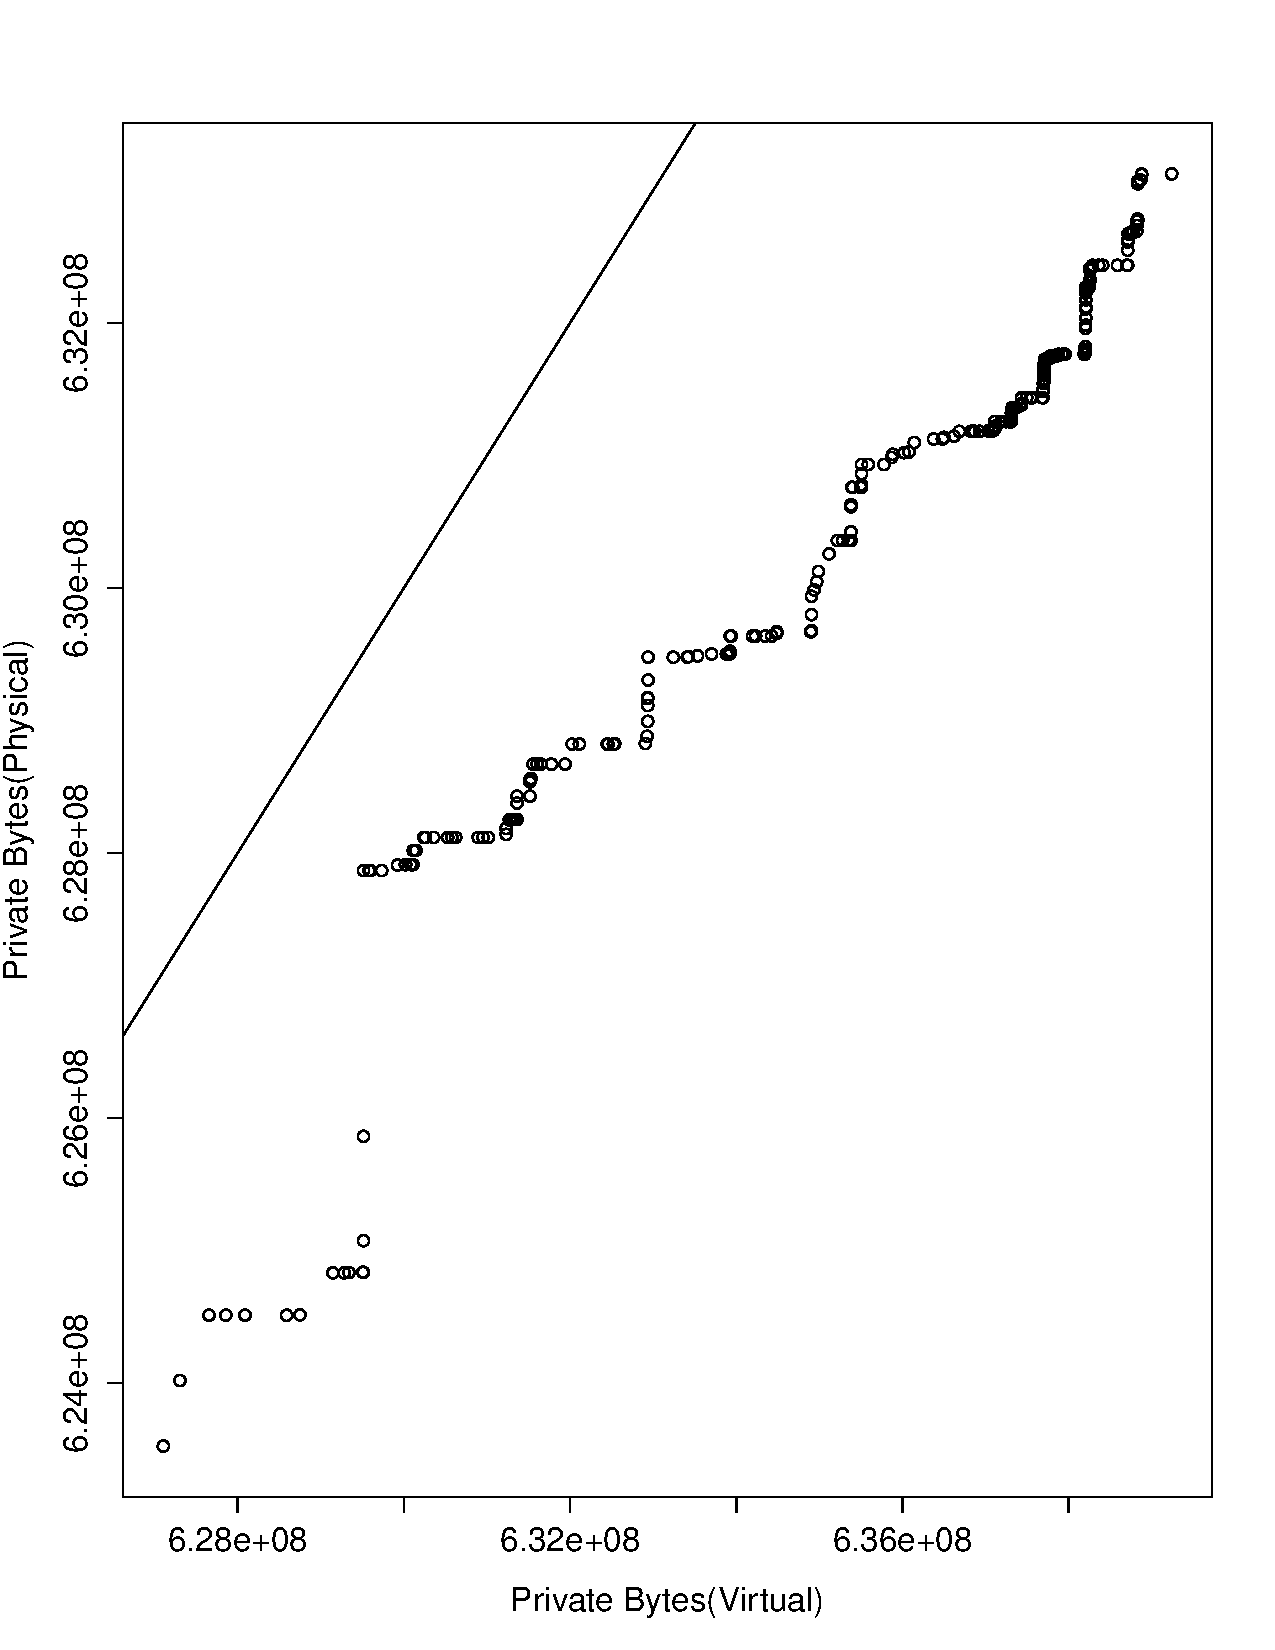
\includegraphics[width=0.7\textwidth]{private_bytes.pdf}
%	\caption{QQ-plot of Private Bytes of Physical vs. Virtual Environment}
%	\captionsetup{justification=centering}
%	\label{fig:Results Table}
%\end{figure}

%\textbf{Approach}: 
%Following our data preprocessing, we decided to use Q-Q plot to identify if there exists a similarity between the distribution of our counters for the dedicated and the virtual server. We divided our metrics into three sub-categories namely \textit{processor, IO and memory}.


\subsection{Examining relationship among performance metrics}

%\textbf{Motivation}: Building on the conclusion from the previous research question, we next address the change in metric correlation values amongst themselves and versus the load. Our goal was to explore whether the change in correlation cross-environments is identical for both of our subject systems. This way we will be able to conclude whether a certain type of discrepancy is always present between the two environments or is it the unstable nature of the performance of subject systems in different environments. 

%Before the software is deployed in a physical environment, the performance analyst relies on the heuristics generated from the virtual environment \cite{foo2010mining}. One of the approaches to detect performance regression is to compare every metric with the previously passed performance test \cite{Shang:2015:ADP:2668930.2688052}. As discussed in our previous research question, most of the performance metrics between two environments do not belong to the similar distribution. 

%As discussed in RQ1, we discovered that our comparison of performance metrics between our physical and virtual environments produced dissimilar results. Our next step was to explore what metrics changed the most 


%As performance testing spans our from handful of hours to several days , the reliability on such exercise is remarkably critical. A recent bug fix or a modification may require a reiteration of performance tests \cite{foo2010mining}. On the contrary, This led us to our next question, that whether the performance assurance activities run on virtual environments can be duplicated.

\noindent \textbf{Approach.} 

We calculate the Spearman's ranking correlation coefficient among all the metrics from each performance test in one environment to study the relationship among these metrics. Then we study whether such correlation coefficient is different between virtual and physical environment. 

First, we compare the changes in correlation between the performance metrics and the system throughput. For example, in one environment, the system throughput may be highly correlated with CPU while in another environment, such correlation is low. In such a case, we would consider the that there exist discrepancy in the correlation coefficient between CPU and the system throughput. Then, for every two metrics, we calculate the absolute difference between the correlation in two environments. For example, if CPU and Memory has a correlation of $0.3$ in virtual environment and $0.5$ in physical environment, we report the absolute difference in correlation as $0.2$ ($|0.3-0.5|$). Since we have 44 metrics in total, we plot a heatmap in order to visualize the 1,936 absolute difference values between every pair of performance metrics. The lighter the color for each block in the heatmap, the larger the absolute difference in correlation a pair of performance metrics have. With the heatmp, we can quickly spot the metrics that have large discrepancy in correlation coefficient. 

%In particular, we 


%We looked for the top 5 metrics which are highly correlated with the load in each of our environments. We used R's \textit{cor} function to determine the Spearman value of the aforementioned associations. 
%Next, we used heat maps to highlight the set of metrics which show a significant change in correlation values amongst themselves.
%The correlation values between the metrics of physical server were stored in matrix A. The correlation values between the metrics of the virtual server were store in matrix B. Matrix Z was the absolute difference between these two matrices. For example the Spearman correlation value for CloudStore's physical server between web server's User Time and database server's IO write/Bytes sec is 0.94. The correlation value for the same pair of metrics in the virtual environment is 0.26. Then the Matrix Z will record a value which is the absolute difference of the aforementioned Spearman values i.e. 0.68. If the metric value has changed significantly, according to the legend, this will be denoted as a 'hot zone' in the heatmap denoted by a lighter gradient of color.

\noindent \textbf{Results.}

\noindent \textbf{The correlation between system throughput and performance metrics changes between virtual and physical environments.} Table~\ref{tab:top10ds2p} presents the top ten metrics with highest correlation to system throughput in the physical environment for DS2. We find that for these ten metrics, the difference in correlation coefficients in virtual and physical environment is up to 0.77 for rank change from X to Y.

\noindent \textbf{There exist differences in correlation among the performance metrics from virtual and physical environments.} Figure~\ref{fig:heatmap} present the heatmap that illustrates the changes in correlation coefficient among the performance metrics from virtual and physical environments. By looking at the heatmap, we can find hotspots (with lighter color), which have larger correlation differences. Due to the limited space, we do not show all the metric names in Figure~\ref{fig:heatmap}. Instead, we enlarge the heatmap by showing one of the hotspots for each subject system in Figure~\ref{fig:heatmap}. We find that the hotspot in DS2 corresponds to the changes in correlation among I/O related metrics. Prior research on virtual machines has similar findings about I/O overheads in virtual machines~\cite{menon2005diagnosing,kraft2011io}.


%\ian{todo: this paragraph maybe useful} Figure 4 and 5 are the heatmaps for the change in correlation values amongst the metrics of two environments. For DS2, figure 4, the hot spots are mostly prevalent between the IO operations, for both the web and database server, cross-environments. This means the correlations amongst IO operations in the physical environment are not the same as the correlation between IO operations in the virtual environment. While CloudStore's heatmap, figure 5, shows that the change in correlation values is not as similar to DS2. Most of the hot spots are scattered across the heatmaps, contrary to DS2 where we can see clusters around most of the IO operations.  We also observed a similar change in correlation values between the processor times and other metrics. This trend may not be as strong as CloudStore's heatmap for DS2, however these changes in values can be found in both of our subject system.

%Table 3-6 are the top five highly correlated metrics with the load. In DS2, most of the IO operations from the web driver are highly correlated with the load in the physical environment. However, the database server is highly correlated than any of the metrics from the web driver in the virtual environment.
%Table 5 and 6 shows a much similar behavior of CloudStore in both the environments.

%We primarily learned that the DS2 IO operations' behavior in one environment are not similar to that of the physical environment. We also learned that the change in nature of correlation cross-environments is non-uniform.
%Figure 4 and 5 are the heatmaps for the change in correlations' values between the metrics of two environments. For DS2, figure 4, 4he hot spots are mostly prevalent between the IO operations cross-environment while CloudStore's heatmap, figure 5, shows that the change in correlation values is not as similar to DS2. Most of the hot spots are scattered across the heatmaps, contrary to DS2 where we can see clusters around most of the IO operations.
\hypobox{The correlations between performance metrics and system load may change considerably between virtual and physical environments. The correlation among performance metrics may also change considerably between virtual and physical environments. The correlations that are related with the I/O metrics have the largest discrepancy. }


\begin{figure*}[tbh]
	\centering
	{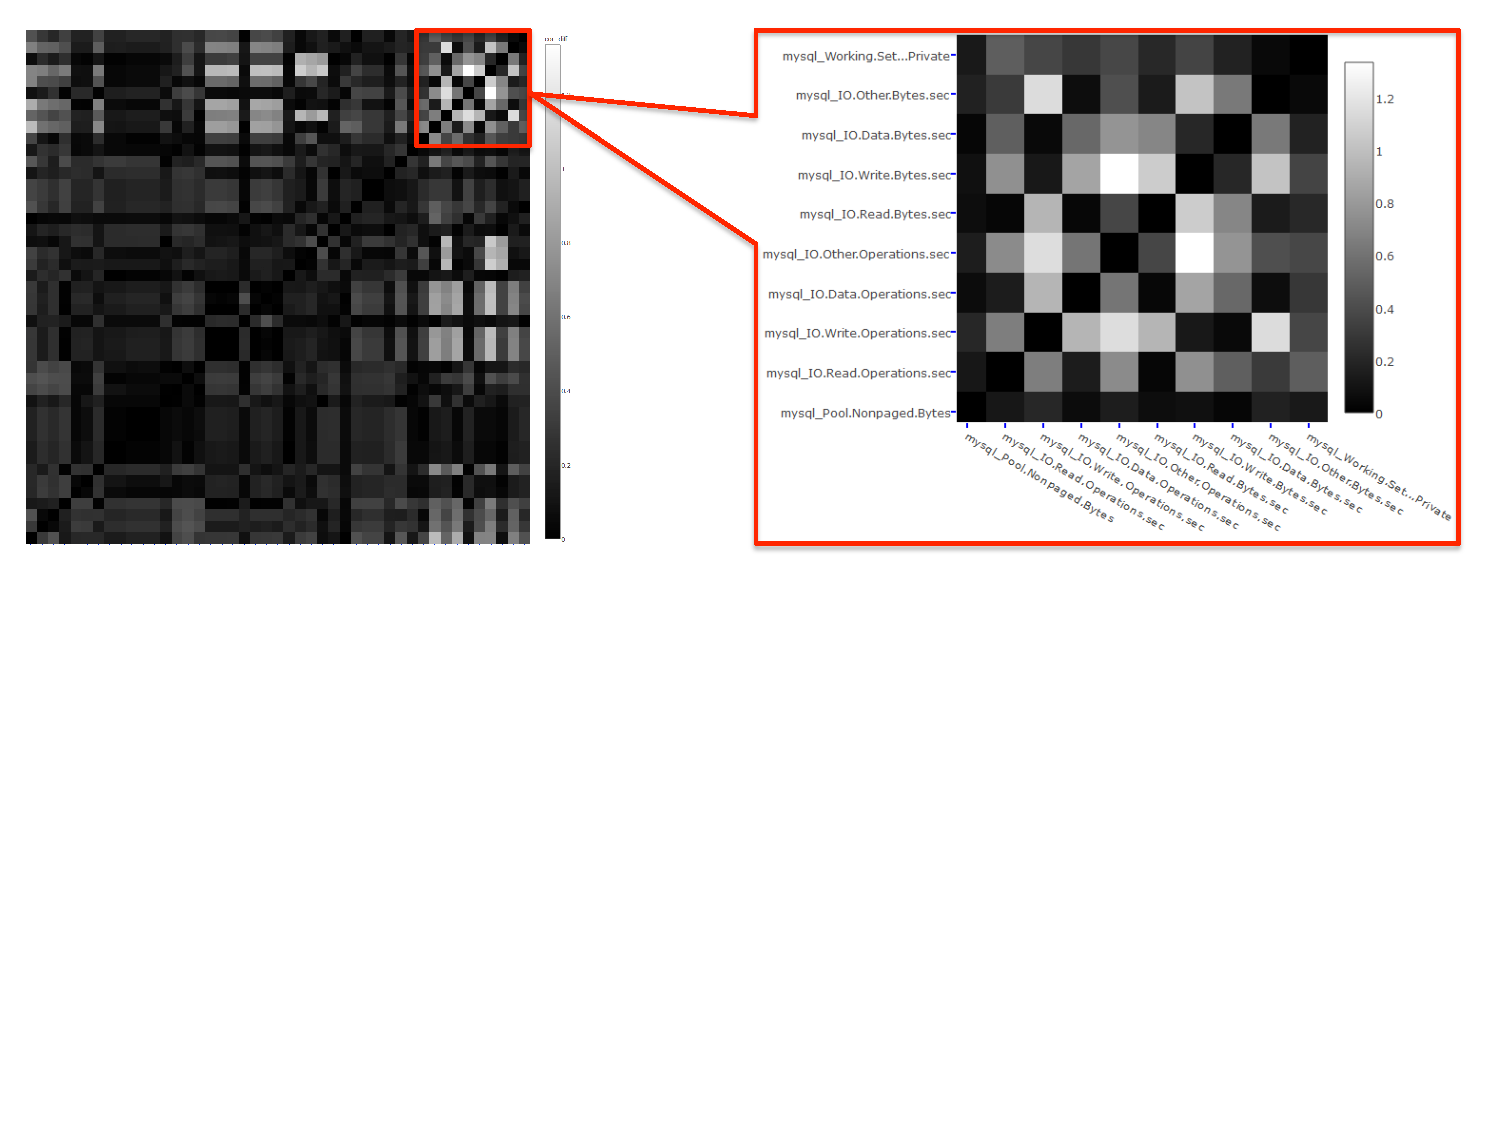
\includegraphics[width=.9\textwidth]{figures/heat}}
	\caption{Heatmap of correlation changes for DS2.}
	%\captionsetup{justification=centering}
	\label{fig:heatmap}
\end{figure*}


%\begin{figure}[tbh]
%	\centering	
%	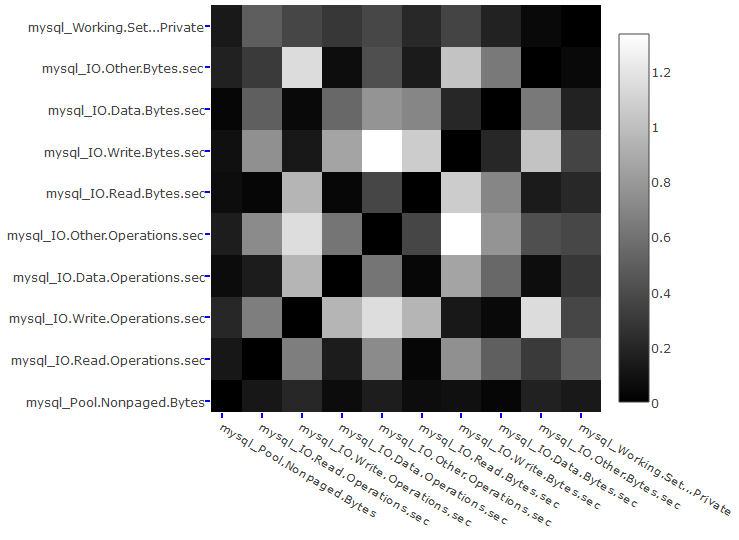
\includegraphics[width=\columnwidth]{figures/ds2_smaller_new.png}
%	\caption{Heatmap: DS2}
%	\captionsetup{justification=centering}
%	\label{fig:heathotds2}
%\end{figure}

%\begin{figure}[tbh]
%	\centering
%	{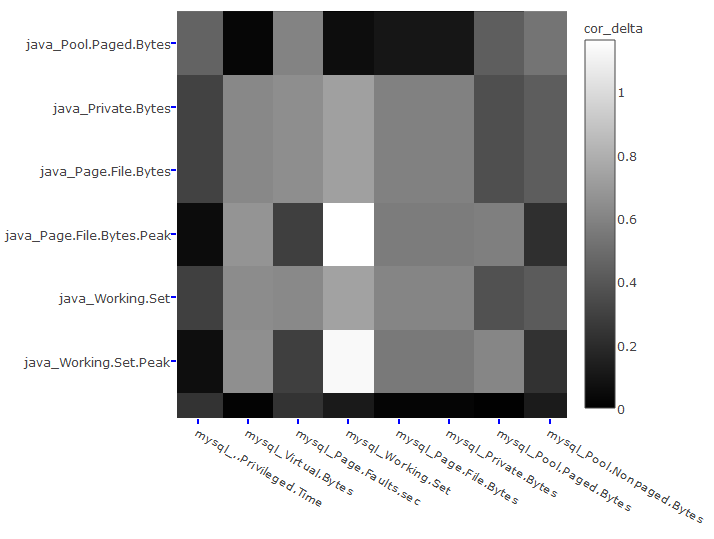
\includegraphics[width=\columnwidth]{figures/cloudstore_heatmap_smaller_new.png}}
%	\caption{Heatmap: CloudStore}
%	%\captionsetup{justification=centering}
%	\label{fig:heathotcs}
%\end{figure}


%\begin{table}[tbh]
%		\centering
%		\caption{DS2: Top 5 highly correlated metrics with load (Physical Server)}
%		\label{resultRQ3}
%		\begin{tabular}{c}
%			\toprule
%			1. Web Server IO Other Operations/sec \\
%			2. Web Server IO Other Bytes/sec \\
%			3. Web Server IO Write Operations/sec \\
%			4. Web Server IO Data Operations/sec \\
%			5. Web Server IO Data Bytes/sec \\
%			
%			\bottomrule             
%		\end{tabular}
%\end{table}


% Please add the following required packages to your document preamble:
% \usepackage{graphicx}
\begin{table}[tbh]
	\centering
	\caption{Top ten metrics with highest correlation coefficient to system throughput in the physical environment for DS2. }
	\label{tab:top10ds2p}
	\resizebox{\columnwidth}{!}{%
	\begin{threeparttable}
	
		\begin{tabular}{|c||c|c|c|c|}
			\hline
			\textbf{Rank} & \textbf{Performance } & \textbf{Coef. } & \textbf{Coef. } & \textbf{Rank in} \\ %\hline
			 & \textbf{ Metrics} & \textbf{PE} & \textbf{VE} & \textbf{VE} \\ %\hline
			\midrule
			1 & Web IO Other Ops/sec & 0.91 & 0.62 & 10 \\ \hline
			2 & Web IO Other Bytes/sec & 0.91 & 0.62 & 12 \\ \hline
			3 & Web IO Write Ops/sec & 0.91 & 0.63 & 9 \\ \hline
			4 & Web IO Data Ops/sec & 0.91 & 0.63 & 8 \\ \hline
			5 & Web IO Write Bytes/sec & 0.90 & 0.62 & 11 \\ \hline
			6 & Web IO Data Bytes/sec & 0.90 & 0.61 & 13 \\ \hline
			7 & DB IO Other Ops/sec & 0.84 & 0.75 & 3 \\ \hline
			8 & DB IO Data Ops/sec & 0.83 & 0.07 & 41 \\ \hline
			9 & DB IO Other Bytes/sec & 0.83 & 0.15 & 40 \\ \hline
			10 & DB IO Read Ops/sec & 0.82 & 0.15 & 39 \\ \hline
		\end{tabular}%
		\begin{tablenotes}
			\item PE in the table is short for physical environment; while VE is short for virtual environment.
		\end{tablenotes}
		\end{threeparttable}
		
	}
	
\end{table}


%\begin{table}[tbh]
%	\centering
%		\caption{DS2: Top 5 highly correlated metrics with load (Virtual Server)}
%		\label{resultRQ3}
%		\begin{tabular}{c}
%			\toprule
%			1. Database Server Handle Count \\
%			2. Database Server Working Set-Peak \\
%			3. Database Server Pool Paged Bytes \\
%			4. Database Server IO Other Operations/sec \\
%			5. Database Server Page File Bytes Peak \\
%			\bottomrule             
%		\end{tabular}
%\end{table}

% Please add the following required packages to your document preamble:
% \usepackage{graphicx}

\begin{comment}
\begin{table*}[tbh]
	\centering
	\caption{DS2: Top 10 highly correlated metrics with load (Virtual Server)}
	\label{my-label}
	\resizebox{\textwidth}{!}{%
		\begin{tabular}{|c||c|c|c|c|}
			\hline
			\textbf{Rank} & \textbf{Performance Metrics} & \textbf{Cor in Virtual Environment} & \textbf{Cor in Physical Environment} & \textbf{Rank in Physical Environment} \\ %\hline
			\midrule
			\midrule
			1 & DB Server Working Set Peak & 0.76 & NA & NA \\ \hline
			2 & DB Server Pool Paged Bytes & 0.75 & 0.30 & 20 \\ \hline
			3 & DB Server IO Other Ops/sec & 0.75 & 0.84 & 7 \\ \hline
			4 & DB Server Virtual Bytes Peak & 0.71 & NA & NA \\ \hline
			5 & DB Server Page File Bytes Peak & 0.71 & NA & NA \\ \hline
			6 & DB Server Working Set & 0.63 & 0.21 & 23 \\ \hline
			7 & DB Server Working Set Private & 0.63 & 0.21 & 24 \\ \hline
			8 & Web Server IO Data Ops/sec & 0.63 & 0.91 & 4 \\ \hline
			9 & Web Server IO Write Ops/sec & 0.63 & 0.91 & 3 \\ \hline
			10 & Web Server IO Other Ops/sec & 0.63 & 1 & 0.91 \\ \hline
		\end{tabular}%
	}
\end{table*}


%\begin{table}[tbh]
%	\centering
%		\caption{CloudStore: Top 5 highly correlated metrics with load (Physical Server)}
%		\label{resultRQ3}
%		\begin{tabular}{c}
%			\toprule
%			1. Database Server IO Other Bytes/sec  \\
%			2. Database Server IO Read Operations/sec   \\
%			3. Database Server IO Read Bytes/sec \\
%			4. Database Server IO Data Operations/sec    \\
%			5. Database Server IO Write Operations/sec \\
%			\bottomrule             
%		\end{tabular}
%\end{table}
%

\begin{table*}[tbh]
	\centering
	\caption{CloudStore: Top 10 highly correlated metrics with load (Physical Server)}
	\label{my-label}
	\resizebox{\textwidth}{!}{%
		\begin{tabular}{|c||c|c|c|c|}
			\hline
			\textbf{Rank} & \textbf{Performance Metrics} & \textbf{Cor in Physical Environment} & \textbf{Cor in Virtual Environment} & \textbf{Rank in Virtual Environment} \\ %\hline
			\midrule
			\midrule
			1 & DB Server IO Other Bytes/sec & 0.98 & 0.73 & 10 \\ \hline
			2 & DB Server IO Read Ops/sec & 0.98 & 0.84 & 7 \\ \hline
			3 & DB Server IO Read Bytes/sec & 0.98 & 0.93 & 5 \\ \hline
			4 & DB Server IO Write Ops/sec & 0.98 & 0.97 & 2 \\ \hline
			5 & DB Server IO Data Ops/sec & 0.98 & 0.92 & 6 \\ \hline
			6 & DB Server IO Data Bytes/sec & 0.98 & 0.96 & 4 \\ \hline
			7 & DB Server IO Write Bytes/sec & 0.98 & 0.96 & 3 \\ \hline
			8 & Web Server IO Other Bytes/sec & 0.98 & 0.68 & 16 \\ \hline
			9 & DB Server IO Other Ops/sec & 0.98 & 0.98 & 1 \\ \hline
			10 & Web Server IO Other Ops/sec & 0.98 & 0.70 & 14 \\ \hline
		\end{tabular}%
	}
\end{table*}


%\begin{table}[tbh]
%	\centering
%		\caption{CloudStore: Top 5 highly correlated metrics with load (Virtual Server)}
%		\label{resultRQ3}
%		\begin{tabular}{c}
%			\toprule
%			1. Database Server IO Other Operations/sec  \\
%			2. Database Server IO Write Operations/sec   \\
%			3. Database Server IO Write Bytes/sec \\
%			4. Database Server IO Data Bytes/sec    \\
%			5. Database Server IO Read Bytes/sec \\
%			\bottomrule             
%		\end{tabular}
%\end{table}

% Please add the following required packages to your document preamble:
% \usepackage{graphicx}
\begin{table*}[tbh]
	\centering
	\caption{CloudStore: Top 10 highly correlated metrics with load (Virtual Server)}
	\label{my-label}
	\resizebox{\textwidth}{!}{%
		\begin{tabular}{|c||c|c|c|c|}
			\hline
			\textbf{Rank} & \textbf{Performance Metrics} & \textbf{Cor in Virtual Environment} & \textbf{Cor in Physical Environment} & \textbf{Rank in Physical Environment} \\ %\hline
			\midrule
	     	\midrule
			1 & DB Server IO Other Ops/sec & 0.98 & 0.98 & 9 \\ \hline
			2 & DB Server IO Write Ops/sec & 0.97 & 0.98 & 4 \\ \hline
			3 & DB Server IO Write Bytes/Sec & 0.96 & 0.98 & 7 \\ \hline
			4 & DB Server IO Data Bytes/sec & 0.96 & 0.98 & 6 \\ \hline
			5 & DB Server IO Read Bytes/sec & 0.93 & 0.98 & 3 \\ \hline
			6 & DB Server IO Data Ops/sec & 0.92 & 0.98 & 5 \\ \hline
			7 & DB Server IO Read Ops/sec & 0.83 & 0.98 & 2 \\ \hline
			8 & DB Server User Time & 0.78 & 0.89 & 22 \\ \hline
			9 & DB Server Processor Time & 0.76 & 0.91 & 21 \\ \hline
			10 & DB Server IO Other Bytes/sec & 0.72 & 0.97 & 1 \\ \hline
		\end{tabular}%
	}
\end{table*}

\end{comment}
\subsection{Building statistical models using performance metrics}
\label{sec:model}
%\textbf{Motivation}: As discussed in earlier work \cite{Shang:2015:ADP:2668930.2688052} \cite{Nguyen:2012:ADP:2188286.2188344}, performance tests require a large dedication of resources as it is carried out just before the system is on the brink of deployment. This gives insufficient time to the performance engineers, leaving them with minimal resources. As a result they leverage on the performance assurance activities carried out in the virtual environment. The motivation behind this research question is to investigate whether the performance models generated from one environment can be applied and held representatives of the other. In essence, this will help the practitioners conclude the reliability of the performance activities carried out in the virtual environment. 
% In practice, this may or may not be appropriate to assume. This also spawns the concept of including the entire set of performance metrics for analysis, which is slipshod and ineffectual. 

\noindent \textbf{Approach. }

We first build statistical models using performance metrics from one environment, then we validate our performance model with the metric values from the same environment and from a different environment.
%\ian{need a figure here.}
\subsubsection{B-1: Reducing counters}

In the first step, we remove redundant performance metrics with low variance in both new and old tests. We first remove performance counters that have zero variance in both versions of the performance tests. We then perform a correlation analysis on the performance metrics. We used the Spearman's ranking correlation coefficient among all performance metrics from in one environment. We find the two performance metrics that have a higher than \ian{what's your threshold} correlation. From these two performance metrics, we remove the metric that have a higher average correlation with all other metrics. We repeating this step until there is no correlation that is higher than \ian{what's your threshold}.

We then perform redundancy analysis~\cite{harrell2001regression} on the performance metrics. The redundancy analysis would consider a performance metric redundant if it can be predicted from a combination of other metrics. We use each performance metric as a dependent variable and use the rest of the metrics as independent variables to build a regression model. We calculate the $R^2$ of each model and if the $R^2$ is larger than a threshold, the current dependent variable (i.e., performance metric) is considered redundant. We then remove the performance metric with the highest $R^2$ and repeat the process until no performance metric can be predicted with $R^2$ higher than the threshold.

\subsubsection{B-2: Building statistical models}

In the second step, we build a build a regression models~\cite{freedman2009statistical} using the performance metrics that are left after the reduction in the first step as independent variables and use the system throughput as dependent variable. Similar models have been build in prior research~\cite{Cohen:2005:CIC:1095810.1095821,xiong2013vperfguard}.

\subsubsection{B-3: Identifying insignificant metrics}
Not all the metrics in the model are statistically significant. Therefore in this step, we only keep the metrics that statistically significantly contribute to the model. We leverage a The \textit{stepwise} function that adds the independent variables one by one to the model to exclude any metrics that not contributing to the model~\cite{RInAction}. 

\subsubsection{B-4: Finalizing statistical models}
After removing all the insignificant metrics, we have all the metrics that significantly contribute to the model. We use these metrics as independent variables to build the final model.

\subsubsection{V-1: Validating model fit}

Before we validate the model with internal and external data, we first examine how good is the model fit. If the models are poorly fit to the data, the our findings from the model may be biased by the noise from the poor model quality. We calculate the $R^2$ of each model. If the model is perfectly fit to the data, the $R^2$ of the model is 1, while a 0 $R^2$ value indicates that the model is completely random. We also would like to estimate the impact that each independent variable has on the model fit. We follow a ``drop one'' approach~\cite{Chambers1990}, which measures the impact of an independent variable on a model by measuring the difference in the performance of models built using: (1) all independent variables (the full model), and (2) all independent variables except for the one under test (the dropped model). A Wald statistic is reported by comparing the performance of these two models. A larger Wald statistic indicates that an independent variable has an larger impact on the model’s performance, i.e., model fit. Similar approach has been leveraged by prior research~\cite{mcintosh2015emse}. We then rank the independent variables by their impact on model fit. 


%After removing any outliers for both of our subject systems, we built our GLM, initially, using all the physical server's metrics. We trained and tested our model on the same server i.e. physical. We then reduced our model, iteratively, using only the metrics that our contributing the most to the model. This was achieved using R's \textit{stepwise} function. The \textit{stepwise} function adds the independent variables one by one to the model to exclude any metrics that not contributing to the model \cite{RInAction}. Once the metrics were automatically selected out on the physical server, we used R's \textit{ANOVA}, or \textit{analysis of deviance} to rank the metrics according to their deviance value. Higher the deviance value for a given performance metric in the model, higher the contribution of the performance metric to the model. This approach was similarly applied to the set of metrics from the virtual server to build a generalized linear model. R's \textit{deviancepercentage} was used to determine the explanatory part or fit of our model. It is used to calculate the percentage of deviance for a given GLM model.

\subsubsection{V-2: Internal validation}

We then validated our models with the performance testing data that is from the same environment. We leverage a standard 10-fold cross validation process, which starts by partitioning the performance data to 10 partitions. We takes one partition (fold) at a time as the test set and trains on the remaining nine partitions~\cite{10foldcross,kohavi1995study}. Similar approach has been adopted by prior performance engineering research~\cite{haroon}. For every data point in the testing data, we calculate the absolute percentage error. For example, for a data point with throughput value 100 requests per minute, if our predicted value is 110 requests per minute, the absolute percentage error is $0.1$ ($\frac{|110-100|}{100}$). After the ten-fold cross validation, we can have a distribution of absolute percentage error for all the data records.

%We partitioned our results into two segments; the explanatory and the predictive part for our models, trailed by applying our model to predict load cross-environments. The explanatory part calculates the percentage of deviance explained by our models i.e. the fit of the model while the predictive part explains the error percentage between the actual and predicted load values. Both of these parts were addressed by building generalized linear models that only incorporated the metrics which were selected via R \textit{stepwise stepwise} or commonly knows as \textit{stepwise} function, from the complete set of metrics from the dataset.


\subsubsection{V-3: External validation}
To evaluate whether the model built using performance testing data in one environment (e.g., virtual environment) can apply to the other environment (e.g., physical environment), we test the model using the data from a different environment. For example, when we build a model using the data from a virtual environment, we test the model using the data from a physical environment. 

Since the performance testing data are generated from different environments, directly applying the data on the model would intuitively generate a large amounts of error. We adopt two approach in order to normalize data in different environments: (1) \textbf{Normalization by deviance.} The first approach we used is the same when we compare distribution of each individual performance counters show in Section~\ref{sec:individual} by calculating the relative deviance of a metric value from its median value (normalization by deviance). (2) \textbf{Normalization by load.} The second approach that we adopt is an approach that is proposed by Nguyen \textit{et al.}~\cite{Nguyen:2012:ADP:2188286.2188344} that uses the load of the system to normalize the performance metric values across different environment. 

%We addressed the presence of a high percentage error by adjusting our virtual environment's metrics to the phsyiscal environment according to the following equation:
%As explained in RQ1, we perceived that our distributions generated by the performance metrics in our environments are not the same. We used R's \textit{predict} to predict our desired set of load, based on the training and testing mentioned in the previous subsections. \textcolor{red}{we used 1-fold cross validation here, necesaary to mention?}


To normalize our metrics, we first build a linear regression model with the one metric as independent variable and the throughput of the system as dependent variable. With the linear regression model in one environment, the metric values can be represented by the system throughput. Then we normalize the metric value by the linear regression from the other environment. The details of the metric transformation is shown as follows:

\begin{equation*}
throughput_{p}= \alpha_{p} \times M_{p} + \beta_{p}
\end{equation*}

\begin{equation*}
throughput_{v}= \alpha_{v} \times M_{v} + \beta_{v}
\end{equation*}

\begin{equation*}
M_{normalized} = \frac{(\alpha_{v} \times M_{v})+\beta_{v}-\beta_{p}}{\alpha_{p}}
	\end{equation*}
where $throughput_{p}$ and $throughput_{v}$ are the system throughput in both environments. $M_{p}$ and $M_{v}$ are the performance metrics from both environments, while $M_{normalized}$ is the metric after normalization. $\alpha$ and $\beta$ are the coefficient and intercept values for the linear regression models. After normalization, we calculate the absolute percentage error for every data record in the testing data.


%The selected counter was chosen on the basis of counters selected by \textit{stepwise}, trained in virtual and tested in physical environment. For every GLM there exists an intercept and a gradient value. We used the aforementioned values and applied them to the metric from the virtual environment as explained by equation 1.
%We also assumed that for each of the metric there will be a gradient and intercept value.




\subsubsection{Identifying model discrepancy}
In order to identify the discrepancy between the models build using data from virtual and physical environment. We compare the two distribution of absolute percentage error from internal and external validation. If the two distribution are significantly different (e.g., the absolute percentage error from internal validation is much lower than that from external validation), the two models are considered to have discrepancy. To be more concrete, in total for each subject system, we ended up four distribution of absolute percentage error: 1) modelling from virtual environment and testing internally (on data from virtual environment), 2) modelling fro virtual environment and testing externally (on data from physical environment), 3) modelling from physical environment and testing internally (on data from physical environment), 2) modelling fro physical environment and testing externally (on data from virtual environment). We compare the distributions 1) and 2) and compare the distributions 3) and 4). Since the first normalization approach (normalization by deviance) will normalize the values to be negative, we performa a min-max normalization on the throughout values before calculating absolute percentage error. In addition, if the observed throughput value after normalization is 0 (when the observed throughput value is the minimum value of both observed and predicted throughput values), we cannot calculate the absolute percentage error for that particular data record. Therefore, we remove the data record if the throughput value after normalization is 0. In our case study, we only remove one data record when performing external validation with model built in physical environment. 




%\textit{Explanatory Power}


%As a result, we had two scenarios per subject system:
%\begin{description}
%	\item[$\bullet$] Trained on physical, tested on physical.
%	\item[$\bullet$] Trained on virtual, tested on virtual.
%\end{description} 

%\textit{Predictive Power}
%\begin{description}
	
	%\paragraph{Cross-Environment}
	
%	The notion behind our predictive approach was to observe the percentage error between the actual and the predicted load. Our first set of predicted values were based on the model trained on the virtual environment's performance metrics and tested on the physical's server metrics. For the dataset of the virtual metrics, we wrote a script in R to remove the metrics that indicated practically zero fluctuation because else they will not have any impact on the GLM. This was trailed by the step to remove any highly correlated metrics and using \textit{stepwise} for every fold \cite{Shihab:2010:UIC:1852786.1852792}. 
	%From the statistical techniques available to validate our model, we used 10-fold cross \cite{kohavi1995study} \cite{10foldcross}.
%	We used mean absolute percentage error (\textit{MAPE}) to measure the error between the predicted and actual load values \cite{mape}. MAPE serves as the percentage measurement of the deviance of our forecasted values from our real values which makes it easier to interpret our results. If the error is 3, we say the forecasted value are off by 3\%. 
	
 %The selection of metrics was based on their presence in the GLMs that were trained in the virtual environment and tested in the physical environment.


 
\noindent \textbf{Results.}

\noindent \textbf{The significant independent variables in the models built by performance testing results in virtual and physical environments are different.} Table~\ref{tab:modelsummaryds2} and \ref{tab:modelsummarycs} show the summary of statistical models built for virtual and physical environments for the two subject systems. We find that all the models have good model fit (66.9\% to 94.6\%). However, some significant independent variables in one model do not appear in the other model. For example, Web Server Virtual Bytes is ranks \# 4 for the model built from physical environment data of CloudStore, while the metric is not significant in the model built from virtual environment data. In fact, none of the significant variables in the model built from virtual environment are related to web server's memory (see Table~\ref{tab:modelsummarycs}). We do observe some performance metrics are significant in both models even with the same ranking. For example, Web Server IO Other Bytes/sec is the \# 1 significant metric for both models built from virtual and physical environments data of DS2 (see Table~\ref{tab:modelsummaryds2}). 

\noindent \textbf{The prediction error illustrates discrepancies between models built by performance testing results in virtual and physical environments.} Although the significant independent variables in the models built by performance testing results in virtual and physical environments are different, the model may have similar prediction results due to correlations between metrics. However, we find that the external prediction errors are higher than internal prediction errors for all four models from virtual and physical environments for the two subject systems. In particular, show in Table~\ref{tab:errors} the prediction errors using normalization based on load is always higher than that of the internal validation. For example, the median absolute percentage error for CloudStore using normalization by load is 632\% and 483\% for the models built in physical environment and virtual environment, respectively; while the median absolute percentage error in interval validation is only 2\% and 10\% for for the models built in physical environment and virtual environment, respectively. However, in some cases, the normalization by deviance can produce low absolute percentage error in external validation. For example, the median absolute percentage error for CloudStore using normalization by deviance is 9\% for the models built in physical environment; while the error from internal validation is 10\%. 

We think the reason is that the normalization based on load, even though is shown to be effective in prior research~\cite{Nguyen:2012:ADP:2188286.2188344}, the approach has assumption of the linear relationship between the performance metric values and the system load, while this may not be true in some performance testing results. For example, Table~\ref{tab:top10ds2p} shows some I/O related metrics do have low correlation with the system load in virtual environments. On the other hand, the normalization based on deviance shows much lower prediction error. We think the reason is that the virtual environments may introduce metric values with high variance. Normalizing based on the deviance controls such variance, leading to the lower prediction errors.

%\ian{todo} Tables 7-10 show the results of our approach. In Table 7, for our subject system DS2, we see that the statistically significant metrics for the GLM from both of our environments are different. The significant of the performance metrics in an GLM is environment dependent. Due to automatic selection of metrics we see a high fit and lower \textit{MAPE} values for our environments. Table 8 shows us the results when the model from the virtual was applied to predict load for the physical server and vice-versa. We observe a an immensely high \textit{MAPE} value for the former while physical-virtual prediction is almost 50\%. This means that the predicted and actual values of the workload have a mean absolute error percentage of almost 50\%. When the same set of metrics from the virtual environment were scaled the MAPE value for DS2 reduces drastically.


%Table 9 shows us the results from CloudStore. Again, the ranks of the metrics that prove to contribute most to the model are not the same compared to both environments. After the data validation, we see a \textit{MAPE} value of almost 16\% for physical server and almost 5\% for virtual. As the GLM was based on automatic selection via \textit{stepwise} regression, we see a high percentage fit for our models. 
%Table 10 shows us the results of cross application of models. A model that was trained on virtual server and tested to predict the workload values for the physical server was off by almost 29\% whereas from physical applied to virtual it was off by 293\%. Similarly, when the metrics were scaled, instead of a an expected decrease in the MAPE value we see that the MAPE jumps from 28.95\% to 276.04\%.

%Not only the \textit{MAPE} values are high when applying models cross environments, they are inconsistent between two environments. We conclude that for both of our subject systems, the models can not directly be applied to predict load for the other environment. We also observed that scaling according to the physical environment may or may not work. This is dependent on the selection of metrics in both of the environments. What might be significant in on of the models may not be applicable to the other model in another environment. 




%We obtained the former equations with the models by training and testing on the respective environments. These equations are derived from the previous work of \cite{Nguyen:2012:ADP:2188286.2188344} Once, the model was constructed we extracted the \(\alpha\) and \(\beta\) values from each model and applied them to scale the virtual environment's metrics accordingly. Equation (1) shows the derived equation through which we scaled the metrics during the process of scaling the counters. 


	%As shown in Table 3, we concluded that most of the contributions to our models are by \textit{DISC IO} and the \textit{CPU}. Inclusion of the aforementioned set of performance metrics gave us a fit percentage closer to the models which included all of the performance metrics. Additionally, the models that were based on the statistically significant metrics ranked by the other environment showed a MAPE value of no more than 7\%. This helped us conclude the metrics that are contributing the most between are environments are overlapping.  
	%The unscaled transfer of metrics generated a \textit{MAPE} value \textbf{40\%} more than that of scaled counters. Our approach successfully identified that the performance metrics generated in the virtual environment can not be taken as the exact reflection of the performance of the system in the physical environment. We also deduced the diversity in environment does impact the regression models and the performance assurance activities. One of the solution to counters this is scaling, however, the error still remains relatively high as shown in Table 2.
	
	%\afterpage{%
	%    \clearpage% Flush earlier floats (otherwise order might not be correct)
	%    \thispagestyle{empty}% empty page style (?)
	%    \begin{landscape}% Landscape page
	%        \centering % Center table
	%        \begin{tabular}{llll}
	%          \begin{table}[thb!]
	%    \begin{center}
	%    \caption{Results}
	%    \label{tab:project_results}
	%            \begin{tabular}{c||cccc}
	%            \toprule
	%            \textbf{Training-Testing}   & \textbf{Physical - Physical} & \textbf{Physical - Virtual} & \textbf{Virtual - Virtual} & \textbf{Virtual - Physical} \\  
	%            \midrule 
	%            \textbf{Ranking}     &       1. IO Read Bytes/sec & 1.IO Read Bytes/sec & 1.User Time  & 1.IO Read Operations/sec \\
	%             &                               2. IO Data Operations/sec & 2. IO Data Operations/sec & 2. IO Read Bytes/sec & 2. IO Read Operations/sec \\
	%             & 3.IO Read Operations/sec & 3.IO Other Bytes/sec & 3. IO Data Operations/sec & 3. IO Other Bytes/sec \\
	%             & 4. IO Other Bytes/sec & 4. IO Read Operations/sec & 4. IO Other Bytes/sec & 4. IO Write Bytes/sec\\
	%             & 5.IO Data Bytes/sec & & 5.Elapsed Time &\\
	%             & 6.Page Faults/sec & & 6.IO Read Operations/sec &\\
	%             & & & 7. Thread Count &\\
	%             & & & 8. IO Write Bytes/sec &\\
	%             & & & 9.IO Write Operations/sec &\\
	%             & & & 10. Working Set &\\
	%             \midrule
	%             \textbf{Fit} & All metrics: 64.1\% & All metrics: 81\% & All metrics: 81\% & All metrics: 63.4\%\\
	%             & Statistically Significant Metrics: 63.5\% & Statistically Significant Metrics: 81\% & Statistically Significant Metrics: 81\% & Statistically Significant Metrics: 63.2\% \\
	%             \midrule
	%             \textbf{MAPE} & 6.17\% & 3.81\% & 3.89\% & 6.14\% \\
	%            \bottomrule             
	%        \end{tabular}
	%    \end{center}
	%\end{table}
	%\\
	%        \end{tabular}
	%        \captionof{table}{Table caption}% Add 'table' caption
	%    \end{landscape}
	%    \clearpage% Flush page
	%}
	
%\end{description}
	
%%\begin{landscape}
%	\begin{table}[tbh]
%		\centering
%			\caption{DS2: Ranking of Performance Counters and Prediction errors}
%			\label{tab:resultRQ1}
%			\resizebox{\columnwidth}{!}{%
%			\begin{tabular}{c||cc}
%				\toprule
%				\textbf{Training-Testing} & \textbf{Physical - Physical} & \textbf{Virtual - Virtual} \\  
%				\midrule 
%				\textbf{Ranking}     & 1. Web Server Privileged Time & 1. Web Server IO Other Bytes/sec \\
%				\\
%				& 2. Database Server User Time & 2. Web Server Page Faults/sec \\
%				\\
%				& 3. Database Server IO Read Bytes/sec & 3.Database Server Working Set-Peak\\
%				\\
%				& 4. Web Server Page Faults/sec & 4. Web Server Handle Count \\
%				\\
%				& 5. Database Server Privileged Time & 5. Database Server IO Data Operations Bytes/sec \\
%				\\
%				& 6. Database Server IO Write Operations Bytes/sec &\\
%				\\
%				& 7. Database Server Pool Paged Bytes &\\
%				\\
%				& 7. Web Server Working Set-Private &\\
%				\\
%				\midrule
%				\textbf{Fit} &  85.80\% &  67.10\% \\
%				\midrule
%				\textbf{MAPE} & 7.02\% & 10.49\% \\
%				\bottomrule             
%		\end{tabular}%
%	}
%	\end{table}
%%\end{landscape}

% Please add the following required packages to your document preamble:
% \usepackage{graphicx}
\begin{table}[tbh]
	\centering
	\caption{Summary of statistical models built for DS2. The metrics listed in the table are the significant independent variables.}
	\label{tab:modelsummaryds2}
	\resizebox{\columnwidth}{!}{%
		\begin{tabular}{|c||c|c|}
			\hline
			\textbf{Environment} & \textbf{Physical} & \textbf{Virtual} \\ %\hline
			\midrule
			\midrule
			\textbf{Ranking} & 1. Web Server IO Other Bytes/sec & 1. Web Server IO Other Bytes/sec \\ \hline
			\textbf{} & 2. Web Server Page Faults/sec & 2. DB server Working Set - Peak \\ \hline
			\textbf{} & 3. DB Server Page Faults/sec & 3. Web Server Virtual Bytes \\ \hline
			\textbf{} & 4. DB Server IO Write Bytes/sec & 4. Web Server Page Faults/sec \\ \hline
			\textbf{} & 5. Web Server IO Read Bytes/sec & 5. DB Server Page Faults/sec \\ \hline
			\textbf{} & 6. DB Server User Time & 6. DB Server IO Data Ops/sec \\ \hline
			\textbf{} & 7. DB Server Pool Paged Bytes &  \\ \hline
			\textbf{} & 8. DB Server Privileged Time &  \\ %\hline
			\midrule
				\textbf{$R^2$}  & 94.6\% & 66.90\% \\ \hline
%			\textbf{MAPE} & 4.00\% & 10.52\% \\ \hline
		\end{tabular}%
	}
\end{table}
%
%	\begin{table}[tbh]
%		\centering
%			\caption{DS2: Prediction errors cross-environments}
%			\label{resultRQ3}
%			\begin{tabular}{c|c}
%				\toprule
%				\textbf{Training - Testing}   & \textbf{MAPE}\\  
%				\midrule 
%				Physical-Virtual       & 49.97\% \\
%				Virtual - Physical        & 6033.16\% \\
%				Virtual - Physical \textbf{(after scaling)}      & 16.04\% \\
%				\bottomrule             
%			\end{tabular}
%	\end{table}


% Please add the following required packages to your document preamble:
% \usepackage{graphicx}
%\begin{table}[tbh]
		%	\centering
		%	\caption{DS2: Prediction errors cross-environments}
		%	\label{my-label}
		%	%\resizebox{\columnwidth}{!}{%
		%		\begin{tabular}{|c|c||c|}
		%			\hline
		%			\textbf{Training} & \textbf{Testing} & \textbf{MAPE} \\ %\hline
		%			\midrule
		%			\midrule
		%			Virtual & Physical & 16.04\% \\ \hline
		%			Phyiscal & Virtual & 25.33\% \\ \hline
		%		\end{tabular}%
		%	%}
		%\end{table}
%	
%	
%	\begin{table}[tbh]
%		\centering
%			\caption{CloudStore: Ranking of Performance Counters and Prediction errors}
%			\label{tab:resultRQ1}
%			\resizebox{\columnwidth}{!}{%
%				\begin{tabular}{c||cc}
%					\toprule
%					\textbf{Training-Testing} & \textbf{Physical - Physical} & \textbf{Virtual - Virtual} \\  
%					\midrule 
%					\textbf{Ranking}     & 1. Web Server Privileged Time & 1. Web Server IO Data Bytes/sec \\
%					\\
%					& 2. Database Server Privileged Time & 2. Database Server User Time \\
%					\\
%					& 3. Web Server Page Faults/sec & 3.Database Server IO Other Bytes/sec\\
%					\\
%					& 4. Web Server Virtual Bytes & 4.Database Server Page Faults/sec\\
%					\\
%					& 5. Database Server Pool Nonpaged Bytes & \\
%					\\
%					& 6. Database Server Page Faults/sec & \\
%					\\
%					& 7. Database Server Page File Bytes &\\
%					\\
%					& 8. Database Server Working Set &\\
%					\\
%					\midrule
%					\textbf{Fit} &  85.20\% &  89.10\% \\
%					\midrule
%					\textbf{MAPE} & 15.75\% & 4.70\% \\
%					\bottomrule             
%				\end{tabular}%
%			}
%	\end{table}
%	%\end{landscape}
%	



\begin{table}[tbh]
	\centering
	\caption{Summary of statistical models built for CloudStore. The metrics listed in the table are the significant independent variables.}
	\label{tab:modelsummarycs}
	\resizebox{\columnwidth}{!}{%
	\begin{tabular}{|c||c|c|}
		\hline
		\textbf{Environment} & \textbf{Physical} & \textbf{Virtual} \\ %\hline
		\midrule
		\midrule
		\textbf{Ranking} & 1. Web Server Privileged Time & 1. Web Server IO Write Ops/sec \\ \hline
		\textbf{} & 2. DB Server Privileged Time & 2. DB Server IO Read Ops/sec \\ \hline
		\textbf{} & 3. Web Server Page Faults/sec & 3. Web Server Privileged Time \\ \hline
		\textbf{} & 4. Web Server Virtual Bytes & 4. DB Server Privileged Time \\ \hline
		\textbf{} & 5. Web Server Page File Bytes Peak & 5. DB Server IO Other Bytes/sec \\ \hline
		\textbf{} & 6. DB Server Pool Nonpaged Bytes & 6. DB Server Pool Nonpaged Bytes \\ \hline
		\textbf{} & 7. DB Server Page Faults/sec &  \\ \hline
		\textbf{} & 8. DB Server Working Set &  \\ %\hline
		\midrule
		\textbf{$R^2$} & 85.30\% & 90.20\% \\ \hline
%		\textbf{MAPE} & 15.63\% & 3.65\% \\ \hline
\end{tabular}%
}
\end{table}

%
%\end{table}
%\begin{table}[tbh]
%	\centering
%	\caption{DS2: Summary of results after scaling}
%	\label{my-label}
%	\resizebox{\columnwidth}{!}{%
%		\begin{tabular}{|c||c|c|c|c|c|c|c|}
%			\hline
%			\textbf{} & \textbf{Min.} & \textbf{1st Qu.} & \textbf{Median} & \textbf{Mean} & \textbf{3rd Qu.} & \textbf{Max.} & \textbf{MAPE} \\ %\hline
%			\midrule
%			\midrule
%			\textbf{P-P} & 1.977e-05 & 1.142e-02 & 2.543e-02 & 3.985e-02 & 5.212e-02 & 3.160e-01 & 4.00\% \\ \hline
%			\textbf{V-V} & 0.0003329 & 0.0370600 & .0859800 & 0.1050000 & 0.1530000 & 0.5428000 & 10.51885\% \\ \hline
%			\textbf{P-V'} & 0.0002277 & 0.0630600 & 0.1257000 & 0.1669000 & 0.2285000 & 0.9199000 & 16.68668\% \\ \hline
%			\textbf{V-P'} & 0.001459 & 0.345300 & 0.440300 & 0.457900 & 0.555600 & 1.562000 & 45.79069\% \\ \hline
%			\textbf{Normalized Data:V(trained)-P(tested)} & 0.00 & 0.09 & 0.20  & 0.27 & 0.34 & 2.82 & 27.31\% \\ \hline
%		\end{tabular}%
%	}
%\end{table}



%
%
%	\begin{table}[tbh]
%		\centering
%			\caption{CloudStore: Prediction errors cross-environments}
%			\label{resultRQ3}
%			\begin{tabular}{c|c}
%				\toprule
%				\textbf{Training - Testing}  & \textbf{MAPE}\\  
%				\midrule 
%				Physical-Virtual       & 293.62\% \\
%				Virtual - Physical      & 28.95\% \\
%				Virtual - Physical \textbf{(after scaling)} & 276.04\% \\
%				\bottomrule             
%			\end{tabular}
%	\end{table}
%	
	
% Please add the following required packages to your document preamble:
% \usepackage{multirow}
% \usepackage{graphicx}
%\begin{table}[tbh]
%	\centering
%	\caption{Prediction errors cross-environments after scaling}
%	\label{my-label}
%	\resizebox{0.6\columnwidth}{!}{%
%		\begin{tabular}{|c||c|c|}
%			\hline
%			\textbf{System} & \textbf{Scaled} & \textbf{MAPE} \\ %\hline
%			\midrule
%			\midrule
%			\multirow{2}{*}{DS2} & Virtual & 16.04\% \\ \cline{2-3} 
%			& Phyiscal & 25.33\% \\ \hline
%			\multirow{2}{*}{CloudStore} & Virtual & 283.06\% \\ \cline{2-3} 
%			& Physical & 69.16\% \\ \hline
%		\end{tabular}%
%	}
%\end{table}	

% Please add the following required packages to your document preamble:
% \usepackage{graphicx}
%
%\end{table}
%\begin{table}[tbh]
%	\centering
%	\caption{DS2: Summary of results after scaling}
%	\label{my-label}
%	\resizebox{\columnwidth}{!}{%
%		\begin{tabular}{|c||c|c|c|c|c|c|c|}
%			\hline
%			\textbf{} & \textbf{Min.} & \textbf{1st Qu.} & \textbf{Median} & \textbf{Mean} & \textbf{3rd Qu.} & \textbf{Max.} & \textbf{MAPE} \\ %\hline
%			\midrule
%			\midrule
%			\textbf{P-P} & 1.977e-05 & 1.142e-02 & 2.543e-02 & 3.985e-02 & 5.212e-02 & 3.160e-01 & 4.00\% \\ \hline
%			\textbf{V-V} & 0.0003329 & 0.0370600 & .0859800 & 0.1050000 & 0.1530000 & 0.5428000 & 10.51885\% \\ \hline
%			\textbf{P-V'} & 0.0002277 & 0.0630600 & 0.1257000 & 0.1669000 & 0.2285000 & 0.9199000 & 16.68668\% \\ \hline
%			\textbf{V-P'} & 0.001459 & 0.345300 & 0.440300 & 0.457900 & 0.555600 & 1.562000 & 45.79069\% \\ \hline
%			\textbf{Normalized Data:V(trained)-P(tested)} & 0.00 & 0.09 & 0.20  & 0.27 & 0.34 & 2.82 & 27.31\% \\ \hline
%		\end{tabular}%
%	}
%\end{table}
%\begin{table}[tbh]
%	\centering
%	\caption{Internal and external prediction errors for both subject systems.}
%	\label{tab:errors}
%	\resizebox{\columnwidth}{!}{%
%		\begin{tabular}{|c||c|c|c|c|c|c|c|}
%			\hline
%			\textbf{} & \textbf{Min.} & \textbf{1st Qu.} & \textbf{Median} & \textbf{Mean} & \textbf{3rd Qu.} & \textbf{Max.} & \textbf{MAPE} \\ %\hline
%			\midrule
%			\textbf{P-P} & 0.00 & 0.01 & 0.02 & 0.03 & 0.05 & 0.3 & 4.00\% \\ \hline
%			\textbf{V-V} & 0.00 & 0.04 & 0.09 & 0.11 & 0.15 & 0.54 & 10.52\% \\ \hline
%			\textbf{P-V'} & 0.00 & 0.06 & 0.13 & 0.17 & 0.23 & 0.92 & 16.67\% \\ \hline
%			\textbf{V-P'} & 0.00 & 0.34 & 0.44 & 0.48 & 0.56 & 1.56 & 45.79\% \\ \hline
%			\textbf{Normalized Data:V(trained)-P(tested)} & 0.00 & 0.09 & 0.20  & 0.27 & 0.34 & 2.82 & 27.31\% \\ \hline
%			%
%			\textbf{Normalized Data:P(trained)-V(tested)} & 0.00 & 0.08 & 0.25  & 0.36 & 0.49 & 13.65 & 35.72\% \\ \hline
%			%
%		\end{tabular}\\
%\end{table}

% Please add the following required packages to your document preamble:
% \usepackage{multirow}
% \usepackage{graphicx}
%\begin{table}[tbh]
%	\centering
%	\caption{Internal and external prediction errors for both subject systems.}
%	\label{tab:errors}
%	\resizebox{\columnwidth}{!}{%
%		\begin{tabular}{|c|c|c|c|c|c|c|c|c|c|}
%			\hline
%			\multicolumn{10}{|c|}{\textbf{DS2}} \\ \hline
%			\textbf{Model Built} & \multicolumn{2}{c|}{\textbf{Validation}} & \multicolumn{1}{c|}{\textbf{Min.}} & \textbf{1st Quart.} & \textbf{Median} & \textbf{Mean} & \textbf{3rd Quart} & \textbf{Max} & \textbf{MAPE} \\ \hline
%			\multirow{3}{*}{\textbf{Virtual}} & \multicolumn{2}{c|}{\textbf{Internal Validation}}  & 0.00 & 0.01 & 0.02 & 0.03 & 0.05 & 0.3 & 4.00\%\\ \cline{2-10} 
%			& \multirow{2}{*}{\textbf{External Validation}} & \textbf{Normalization by Deviance} & 0.00 & 0.08 & 0.25  & 0.36 & 0.49 & 13.65 & 35.72\%  \\ \cline{3-10} 
%			&  & \textbf{Normalization by Load} &0.00 & 0.34 & 0.44 & 0.48 & 0.56 & 1.56 & 45.79\% \\ \hline
%			\multirow{3}{*}{\textbf{Physical}} & \multicolumn{2}{c|}{\textbf{Internal Validation}} & 0.00 & 0.04 & 0.09 & 0.11 & 0.15 & 0.54 & 10.52\%   \\ \cline{2-10} 
%			& \multirow{2}{*}{\textbf{External Validation}} & \textbf{Normalization by Deviance}& 0.00 & 0.09 & 0.20  & 0.27 & 0.34 & 2.82 & 27.31\%  \\ \cline{3-10} 
%			&  & \textbf{Normalization by Load}  & 0.00 & 0.06 & 0.13 & 0.17 & 0.23 & 0.92 & 16.67\%   \\ \hline
%		\end{tabular}
%\end{table}		
% Please add the following required packages to your document preamble:
% \usepackage{multirow}
% \usepackage{graphicx}
\begin{table*}[tbh]
	\centering
	\caption{Internal and external prediction errors for both subject systems}
	\label{tab:errors}
	\resizebox{\textwidth}{!}{%
		\begin{tabular}{|c||c|c|c|c|c|c|c|c|c|}
			\hline
			\multicolumn{9}{|c|}{\textbf{DS2}} \\ \hline
			\textbf{Model Built} & \multicolumn{2}{c|}{\textbf{Validation}} & \textbf{Min.} & \textbf{1st Quart.} & \textbf{Median} & \textbf{Mean} & \textbf{3rd Quart} & \textbf{Max}\\ %\hline
			\midrule
			\midrule
			\multirow{3}{*}{\textbf{Physical}} & \multicolumn{2}{c|}{\textbf{Internal Validation}} & 0.00 & 0.01 & 0.02 & 0.03 & 0.05 & 0.30 \\ \cline{2-9} 
			& \multirow{2}{*}{\textbf{External Validation}} & \textbf{Normalization by Deviance} & 0.00 & 0.08 & 0.25 & 0.36 & 0.49 & 13.65 \\ \cline{3-9} 
			&  & \textbf{Normalization by Load} & 0.00 & 0.34 & 0.44 & 0.48 & 0.56 & 1.56  \\ \hline
			\multirow{3}{*}{\textbf{Virtual}} & \multicolumn{2}{c|}{\textbf{Internal Validation}} & 0.00 & 0.04 & 0.09 & 0.11 & 0.15 & 0.54 \\ \cline{2-9} 
			& \multirow{2}{*}{\textbf{External Validation}} & \textbf{Normalization by Deviance} & 0.00 & 0.09 & 0.20 & 0.27 & 0.34 & 2.82  \\ \cline{3-9} 
			&  & \textbf{Normalization by Load} & 0.00 & 0.06 & 0.13 & 0.17 & 0.23 & 0.92 \\ \hline
		\end{tabular}%
	}
%\end{table*}

\vspace{2ex}
% Please add the following required packages to your document preamble:
% \usepackage{multirow}
% \usepackage{graphicx}
%\begin{table*}[]
	\centering
	\resizebox{\textwidth}{!}{%
		\begin{tabular}{|c||c|c|c|c|c|c|c|c|}
			\hline
			\multicolumn{9}{|c|}{\textbf{CloudStore}} \\ \hline
			\textbf{Model Built} & \multicolumn{2}{c|}{\textbf{Validation}} & \textbf{Min.} & \textbf{1st Quart.} & \textbf{Median} & \textbf{Mean} & \textbf{3rd Quart} & \textbf{Max}\\ \midrule
			\midrule
			\multirow{3}{*}{\textbf{Physical}} & \multicolumn{2}{c|}{\textbf{Internal Validation}} & 0.00 & 0..05 & 0.10 & 0.16 & 0.18 & 2.68\\ \cline{2-9} 
			& \multirow{2}{*}{\textbf{External Validation}} & \textbf{Normalization by Deviance} & 0.00 & 0.04 & 0.09 & 0.17 & 0.17 & 2.29  \\ \cline{3-9} 
			&  & \textbf{Normalization by Load} & 2.90 & 5.14 & 6.32 & 7.75 & 8.08 & 51.33 \\ \hline
			\multirow{3}{*}{\textbf{Virtual}} & \multicolumn{2}{c|}{\textbf{Internal Validation}} & 0.00 & 0.01 & 0.03 & 0.04 & 0.05 & 0.50  \\ \cline{2-9} 
			& \multirow{2}{*}{\textbf{External Validation}} & \textbf{Normalization by Deviance} & 0.00 & 0.03 & 0.07 & 0.11 & 0.13 & 1.00  \\ \cline{3-9} 
			&  & \textbf{Normalization by Load} & 4.07 & 4.64 & 4.83 & 5.13 & 5.10 & 33.36  \\ \hline
		\end{tabular}%
	}
\end{table*}


\hypobox{The statistical models built by performance testing results in virtual and physical environments have discrepancy. The external prediction errors are higher than internal prediction errors, showing that one cannot apply the models from one environment on data from another environment. Normalizing the performance metrics by deviance may reduce minimize such discrepancy and reduce the external prediction error. Practitioners may consider normalize the performance testing result data from virtual environment by deviance before analysis. }

%		\begin{tabular}{|c||c|c|c|c|c|c|c|}
%			\hline
%			\textbf{} & \textbf{Min.} & \textbf{1st Qu.} & \textbf{Median} & \textbf{Mean} & \textbf{3rd Qu.} & \textbf{Max.} & \textbf{MAPE} \\ %\hline
%			\midrule
%			\textbf{P-P} & 0.00 & 0.05 & 0.10 & 0.16 & 0.18 & 2.68 & 15.63\% \\ \hline
%			\textbf{V-V} & 0.00 & 0.01 & 0.03 & 0.04 & 0.05 & 0.50 & 3.65\% \\ \hline
%			\textbf{P-V'} & 4.07 & 4.64 & 4.83 & 5.13 & 5.10 & 33.36 & 513.00\% \\ \hline
%			\textbf{V-P'} & 2.90 & 5.14 & 6.32 & 7.75 & 8.08 & 51.33 & 774.75\% \\ \hline
%			\textbf{Normalized Data:V(trained)-P(tested)} & 0.00 & 0.03 &  0.07  & 0.11 & 0.13 & 1.00 & 10.73\% \\ \hline
%			%
%			\textbf{Normalized Data:P(trained)-V(tested)} &  0.00 &  0.04 & 0.09  &  0.17 & 0.17 & 2.29  & 17.21\% \\ \hline
%			%
%		\end{tabular}%
%%	}
%\end{table*}



%We retested our virtual and physical environments with a same set of load. As this experiment was a replica of our previous research question, our approach was based on the same lines. After obtaining the performance metrics, we preprocessed our data where every record represented the load and performance metrics generated for a minute. We removed the first thirty entries, which represented first thirty minutes in our tests to remove any noise.  After the preprocessing phase we had three set of metrics for every environment. We labeled one of them as the \textit{baseline metrics} and the rest as \textit{reference metrics 1} and \textit{reference metrics 2}. Succeedingly, these six datasets were imported in R for further analysis.
%To draw conclusion and validate the findings, firstly we removed any metric that showed no variance. This is pursued by removing metrics which are highly correlated with other metrics in the same data set, for example \textit{Processor Time} and \textit{Privileged Time}. We, then, train our data bolstered by the generalized linear model. \textit{Stepwise Regression} is used to filter the metrics which do not contribute to our model. The metrics are added one by one to until no further contribution is made to the model.  \cite{RInAction}. We trained our model with the set of \textit{baseline metrics} and tested our model by predicting the load for the \textit{reference metrics 1} and \textit{reference metrics 2} . We trained iteratively on the rest of the sets of metrics and tested for the remaining two sets of metrics. We repeated this approach for both of our environments.
%We calculated the accuracy of our approach by the \textit{mean absolute percentage error} where the absolute difference of real and predicted values is divided by the real values followed by taking the mean. \cite{perfmon}

%\textbf{Results}:  We observed that \textit{MAPE} values for majority of our experiments run on physical environment fell under \textbf{30\%} while for the virtual the values were more than 200\%. 
%We also concluded that because of the presence of the noise and the irregular behavior of the virtual environment, the experiments did not produce exact similar set of results. The difference in behavior was based on inconsistent \textit{User Time} and \textit{DISC IO} operations. This lead our to our next question that whether the performance testing done in virtual environment can be calibrated and applied to the physical environment, as profoundly practiced in the field of performance testing.
